\clearpage

\section{Vista de Desarrollo}

\textbf{Business Logic}: Contiene la lógica de negocio asociada a las consultas definidas en el alcance. Aquí se implementan las reglas para filtrar, agrupar, unir y consolidar datos, de manera independiente de la infraestructura subyacente.

\textbf{Processing Nodes}: Incluye las implementaciones de los distintos nodos de procesamiento (Select, Group, Join, Result). Cada nodo ejecuta tareas específicas del pipeline y se comunica con otros a través del middleware.

\textbf{Type Handlers}: Define cómo se va a comportar un nodo en función de la consulta que se está ejecutando en el.

\textbf{Middleware}: Proporciona la abstracción de comunicación entre nodos mediante un modelo orientado a colas. Se asegura de la entrega confiable de mensajes, la asincronía y la tolerancia a fallos.

\textbf{State Storage}: Almacenamiento intermedio para nodos con estado (Group y Join). Garantiza que los datos parciales se conserven mientras se procesan.

\textbf{Result Storage}: Repositorio persistente para almacenar los resultados finales, asociados a cada consulta y cliente mediante el requestId.

\textbf{Routing}: Encargado de dirigir cada mensaje hacia el nodo o cola correspondiente, aplicando estrategias de hash y balanceo de carga.

\textbf{Business Protocol}: Define el contrato de comunicación entre cliente y servidor (registro de consultas, consulta de resultados, manejo de identificadores).

\textbf{Task Protocol}: Describe cómo se representan, envían y reciben las tareas de procesamiento entre nodos. Incluye metadatos como tipo de consulta, identificador de cliente y partición.

\textbf{Data Protocol}: Normaliza el formato de los datos transaccionales y de negocio (transacciones, usuarios, productos, sucursales) que circulan en el sistema.

\textbf{Byte Protocol}: Capa más baja de comunicación, que define la serialización y deserialización de los mensajes para su envío eficiente a través del middleware.

\vfill
\begin{figure}[H]
    \centering
    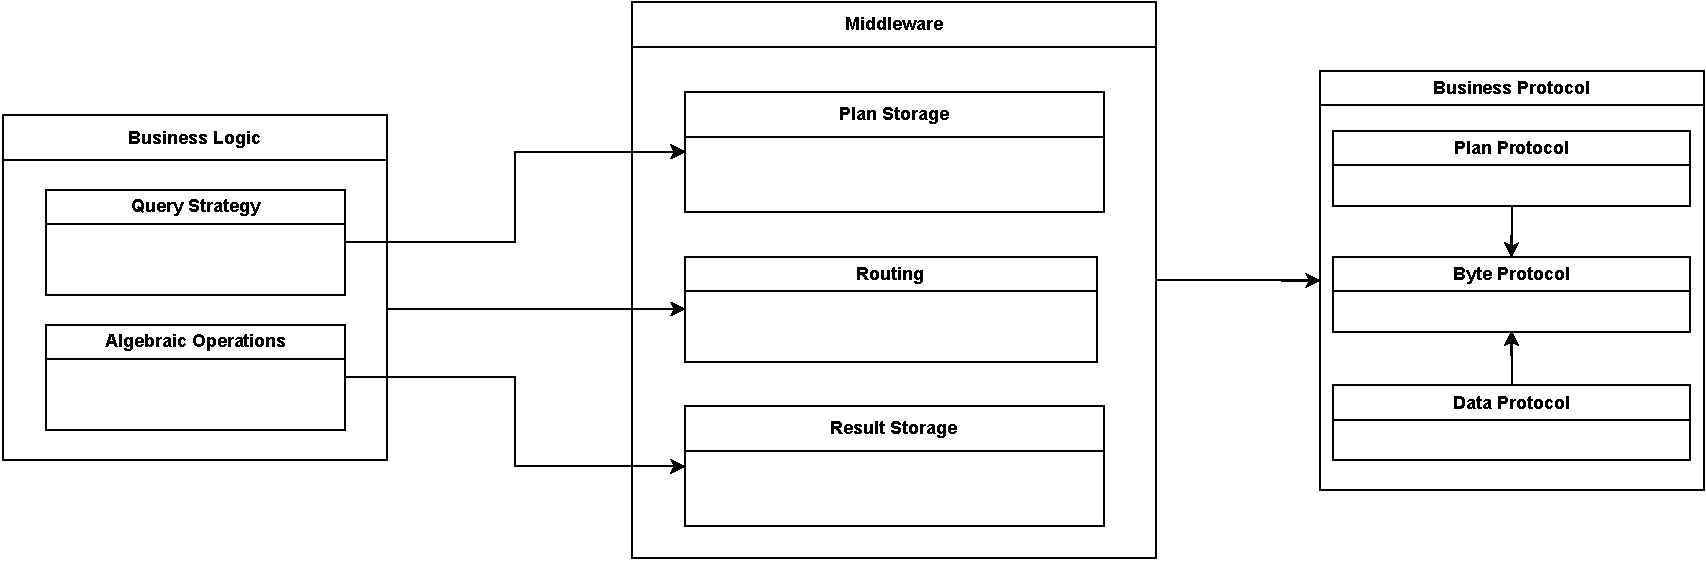
\includegraphics[width=1\textwidth]{img/paquetes.pdf}
    \caption{Diagrama de paquetes}
\end{figure}
\vfill